\documentclass{article}
\usepackage[utf8]{inputenc}
\usepackage{graphicx}
\usepackage{amsmath}
\usepackage{caption}
\usepackage{hyperref}
\usepackage{geometry}
\usepackage{lmodern}
\usepackage{verbatim}
\usepackage{listings}
\lstset{basicstyle=\ttfamily\footnotesize, breaklines=true}
\geometry{margin=2.5cm}

\title{Percolation Project}
\author{Anaya Lizarazo, Bryan Johan; Pinilla Correa, Santiago \& Torres Otálora, Erick}
\date{\today}

\begin{document} 

\maketitle

\section{Introducción}

La percolación es un fenómeno físico y matemático que describe el comportamiento colectivo de elementos conectados en una red, lo cual puede servir para simular el movimiento de fluidos en medios porosos. En este proyecto se estudia el modelo de percolación porosa por sitios sobre una red cuadrada bidimensional de tamaño \( L \times L \). Este modelo consiste en recorrer cada uno de los sitios de la matriz y ocuparlo con una probabilidad \( p \). A partir de esta ocupación aleatoria, se identifican los conglomerados de sitios vecinos ocupados, conocidos como \emph{clusters}.

Para el reconocimiento eficiente de estos clusters se implementó el algoritmo de Hoshen-Kopelman, que permite etiquetar de manera rápida y sin redundancias los distintos conglomerados conectados de la matriz. Con esta información es posible determinar si existe un cluster que conecta los bordes opuestos de la red, es decir, si el sistema \emph{percola}.

En la figura \ref{fig:lattice_clusters} se ilustran dos representaciones de una red: una antes de identificar los clusters en donde los sitios ocupados se representan con 1 y otra después de aplicar el algoritmo de Hoshen-Kopelman, donde cada cluster ha sido etiquetado y representado con un color diferente.

\begin{figure}[h]
    \centering
    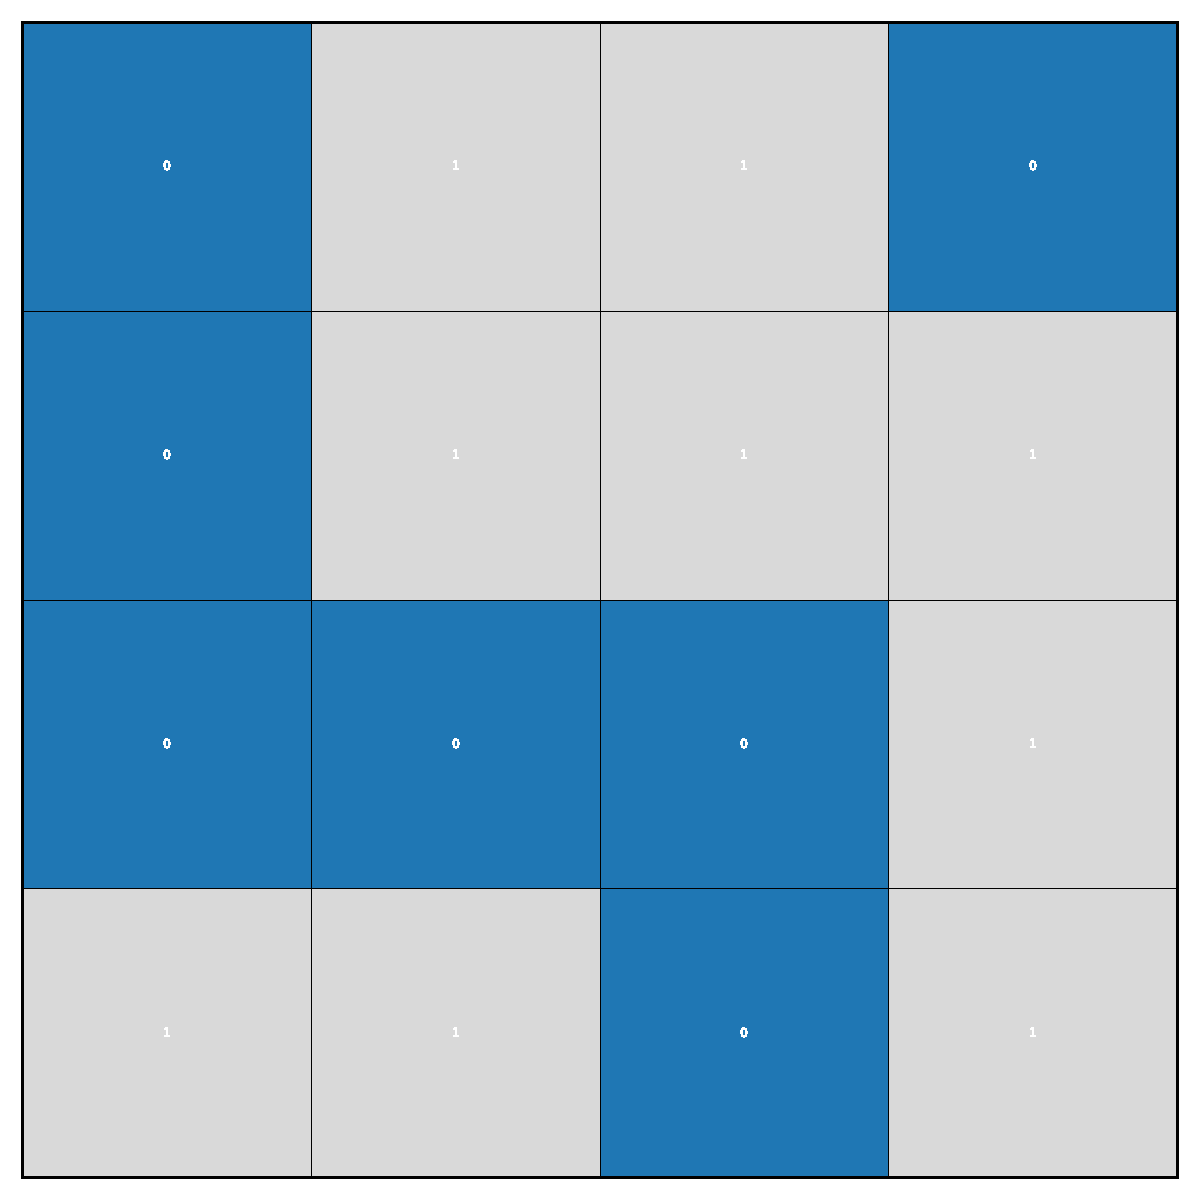
\includegraphics[width=0.45\textwidth]{figures/lattice.pdf}
    \hfill
    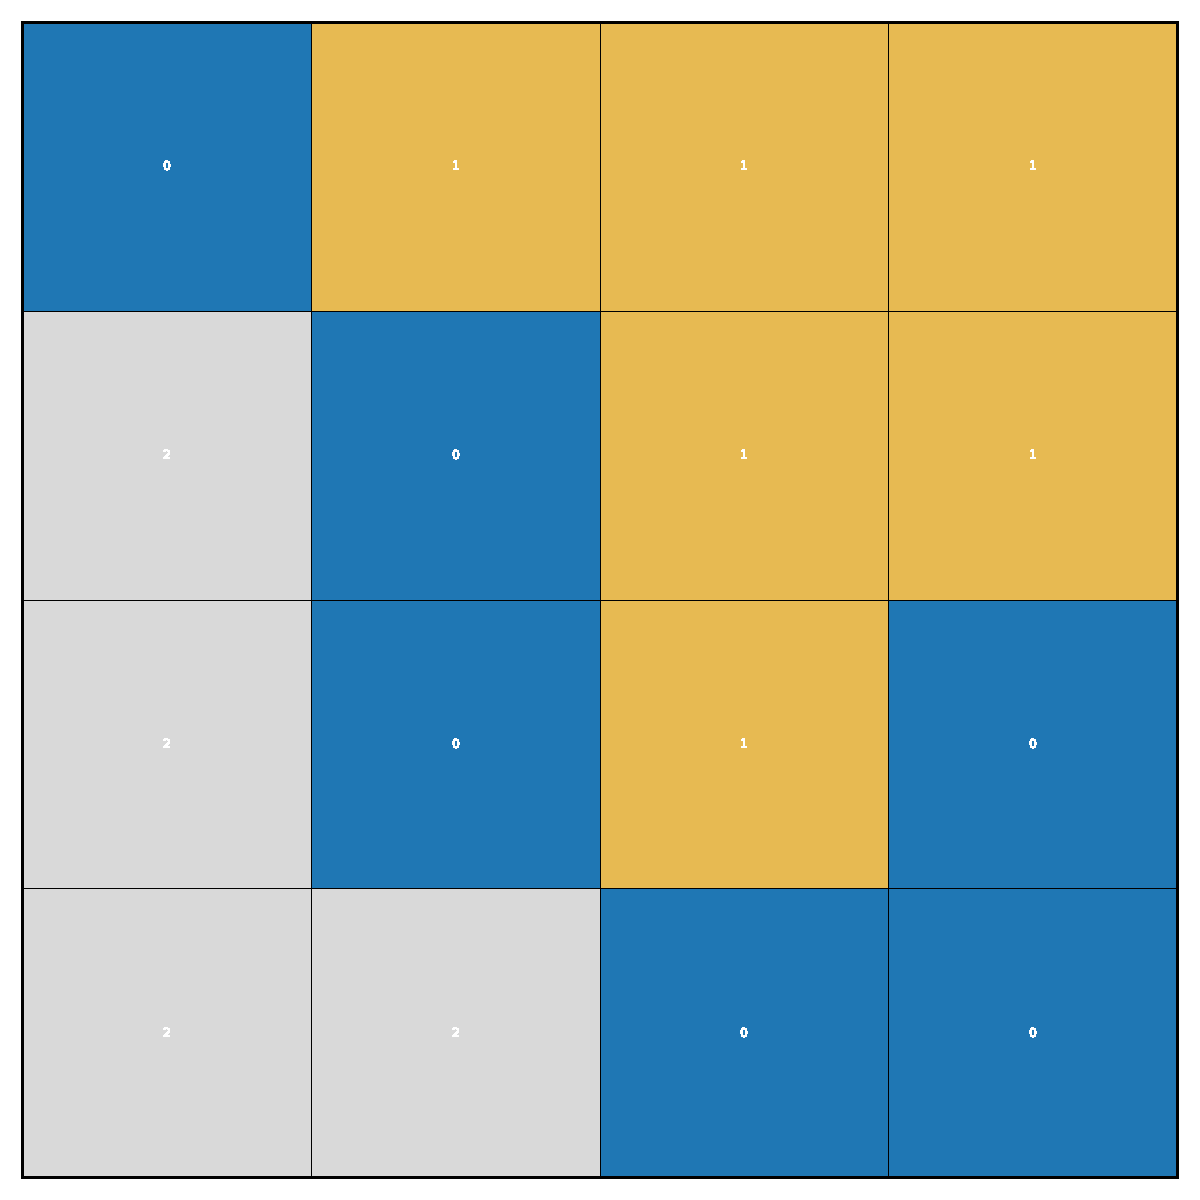
\includegraphics[width=0.45\textwidth]{figures/clusters.pdf}
    \caption{(Izquierda) Lattice de tamaño \( L \times L \) con ocupación aleatoria según probabilidad \( p \). (Derecha) Identificación de clusters mediante el algoritmo de Hoshen-Kopelman.}
    \label{fig:lattice_clusters}
\end{figure}
En el límite termodinámico (\(L \to \infty\)), se define una probabilidad crítica \(p_{c}\). Por debajo de este umbral (\(p < p_{c}\)), no existe clúster percolante de tamaño macroscópico, mientras que para \(p \ge p_{c}\) aparece con probabilidad uno un clúster de tamaño infinito que conecta la red.

El objetivo de este artículo es estudiar el comportamiento de la probabilidad de percolación y del tamaño del cluster percolante en función de los parámetros \(L\) y \(p\), con el fin de comprobar las predicciones teóricas de la teoría de percolación. Además, se analizará la eficiencia del código implementado para distintos niveles de optimización, empleando herramientas de profiling como \texttt{gprof} y \texttt{perf}, con el propósito de identificar posibles optimizaciones y mejorar el rendimiento computacional en la simulación de redes percolates.


\section{Resultados de Percolación}

A continuación se presentan los resultados numéricos obtenidos para la probabilidad de percolación y el tamaño promedio del clúster percolante más grande (normalizado con el tamaño del sistema \( L \times L \)) en función de la probabilidad de llenado \(p\) y para distintos tamaños de red \(L = 16,\,32,\,64,\,128,\,256,\,512\). Dado que se trata de una probabilidad y de un tamaño promedio, se ejecutó el programa 10 veces para poder realizar la estadística sobre estos resultados.

En la Figura \ref{fig:perc_prob} se muestra la probabilidad de percolación \(P(L,p)\) frente a \(p\). Cada curva corresponde a un tamaño \(L\) distinto. Se observa que, para valores bajos de \(p\), la probabilidad de que exista un clúster que conecte bordes opuestos es cero, mientras que al incrementarse \(p\) la probabilidad crece en el intervalo \(p\in(0.5, 0.6)\) para despues ser uno. Además, a medida que \(L\) aumenta, la transición se vuelve más pronunciada y la curva se desplaza hacia el valor crítico \(p_c \approx 0.6\). Este comportamiento es consistente con la teoría de percolación en sistemas finitos, pues la transición es abrupta con \(L\) grande, acercándose a una función escalón en el límite termodinámico.

\begin{figure}[h]
    \centering
    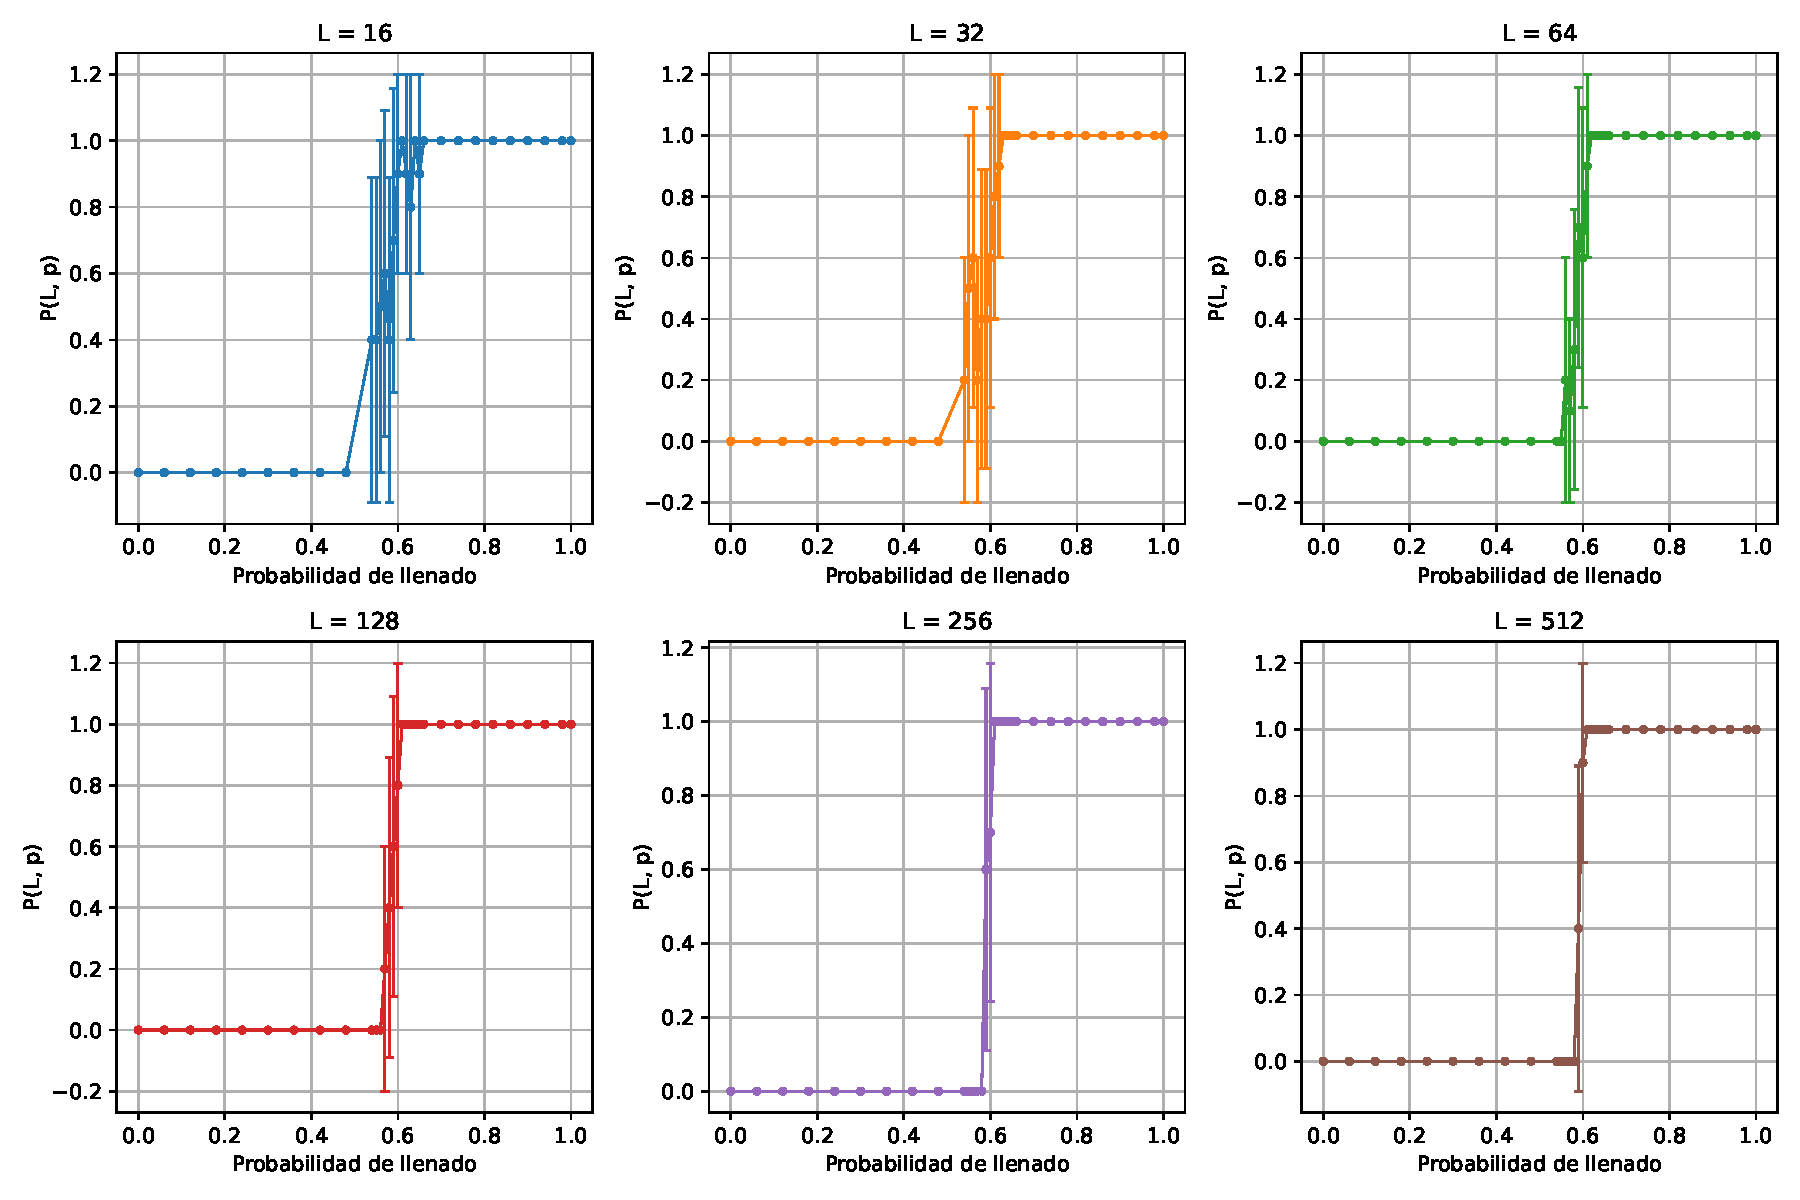
\includegraphics[width=1.0\textwidth]{figures/Perc_prob.pdf}
    \caption{Probabilidad de percolación \(P(L,p)\) frente a la probabilidad de llenado \(p\), para redes cuadradas de tamaño \(L = 16,\,32,\,64,\,128,\,256,\,512\). Se observa una transición en la probabilidad de percolación que se hace más pronunciada al aumentar \(L\).}
    \label{fig:perc_prob}
\end{figure}

Por otro lado, en la Figura \ref{fig:size} se grafica el tamaño promedio del clúster percolante más grande normalizado en función de \(p\). No hay casi datos para \(p\) por debajo del umbral crítico \(p_c\) dado que en estos casos es muy poco probable que se presente percolación (no hay clúster macroscópico). Para los valores de \(p\) toamdos en cuenta, se observa un crecimiento pronunciado cerca de \(p_c\) y posteriormente un crecimiento lineal de \(S(L,p)\) hasta llegar al tamaño del sistema con \(p = 1\) cómo es esperado. Igualmente, el punto de inflexión en donde comienza un crecimiento lineal se da aproximadamente para un tamaño de aproximadamente el 60\% del sistema para todos los valores de L. Sin embargo, conforme \(L\) crece la varianza en los datos disminuye y se obtiene una curva suave, acercandose al caso ideal del limite termodinámico.

\begin{figure}[h]
    \centering
    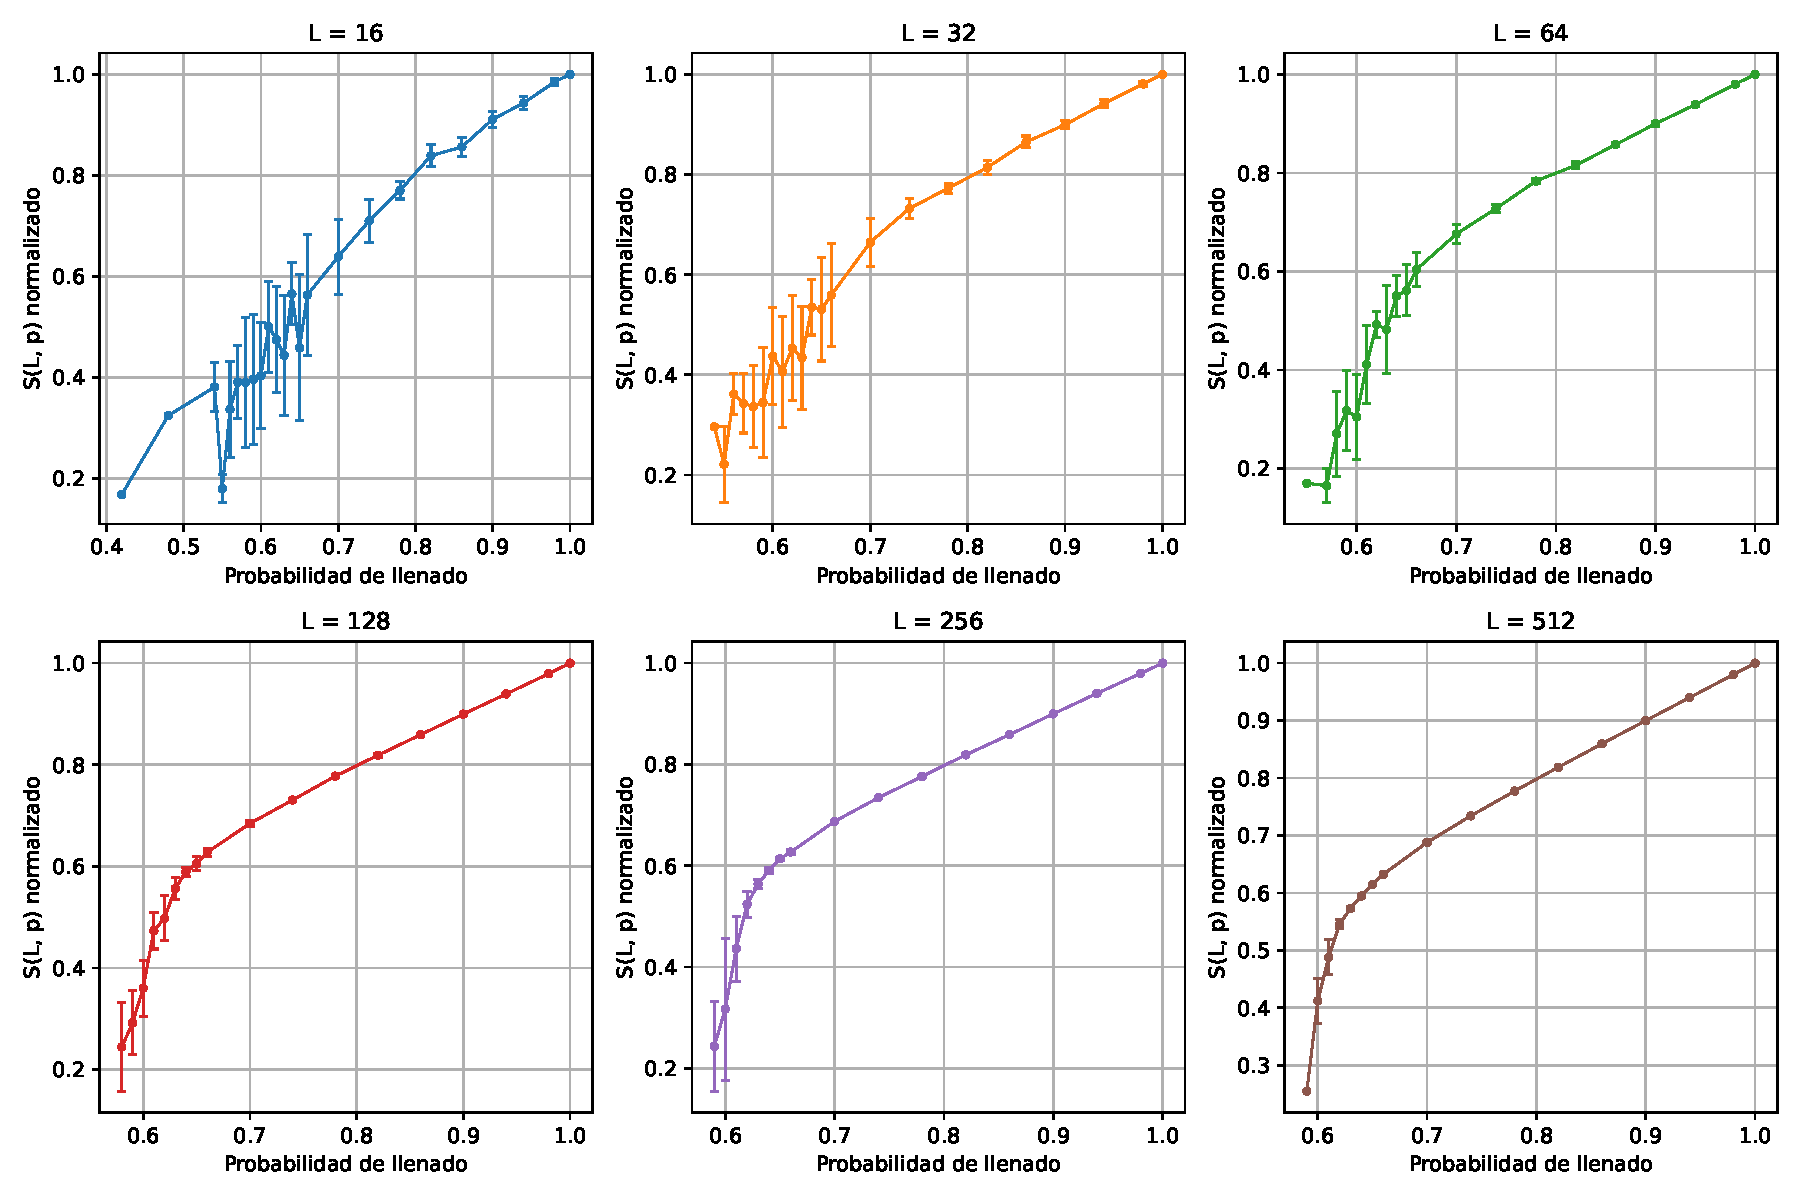
\includegraphics[width=1.0\textwidth]{figures/Size.pdf}
    \caption{Tamaño promedio del clúster percolante más grande normalizado, \(S(L,p) = ( \text{tamaño del clúster mayor} ) / L^2\), frente a la probabilidad de llenado \(p\), para redes cuadradas de tamaño \(L = 16,\,32,\,64,\,128,\,256,\,512\). Se aprecia el crecimiento pronunciado de \(S\) alrededor del umbral crítico.}
    \label{fig:size}
\end{figure}

\section{Análisis profiling}

\subsection{Niveles de optimización}
Para evaluar el impacto de los distintos niveles de optimización del compilador en el rendimiento de nuestro programa de percolación, compilamos el código con las banderas \textit{-O0}, \textit{-O1}, \textit{-O2}, \textit{-O3} y \textit{-Ofast}. A continuación, la Figura~\ref{fig:opt_levels} muestra el tiempo de ejecución medido (en milisegundos) para diferentes tamaños de red \(L\) y la probabilidad de llenado \(p = 0.6\) cercana a la probabilidad crítica.

\begin{figure}[h]
    \centering
    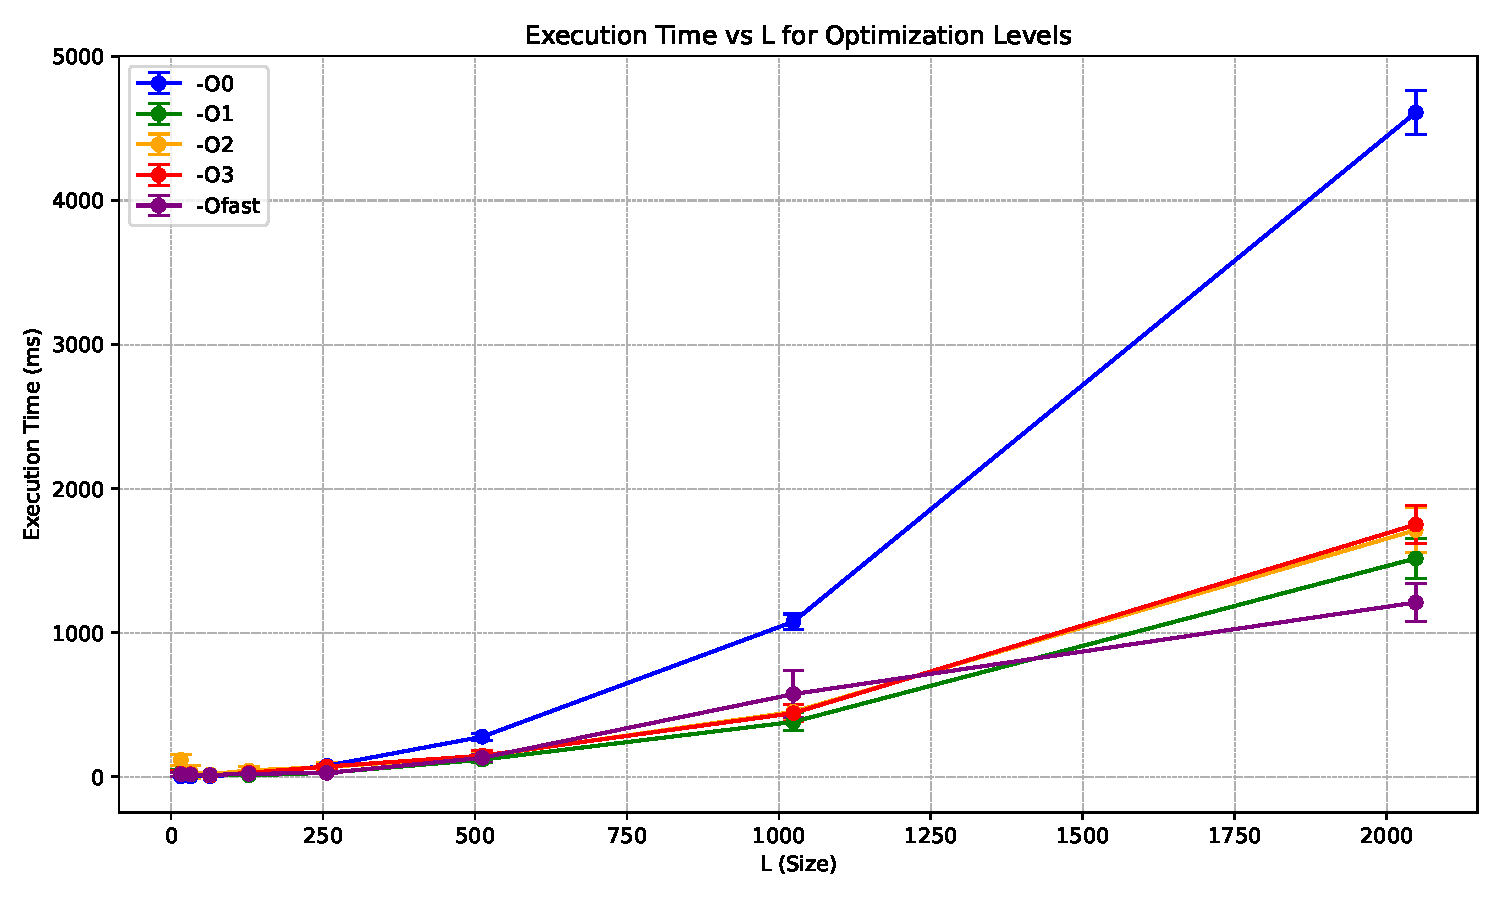
\includegraphics[width=1.0\textwidth]{figures/opti_comparison.pdf}
    \caption{Tiempo de ejecución del programa de percolación en función del tamaño de la red \(L\), compilado con distintos niveles de optimización: \textit{-O0} (sin optimizar), \textit{-O1}, \textit{-O2}, \textit{-O3} y \textit{-Ofast}.}
    \label{fig:opt_levels}
\end{figure}

En general, se observa que el tiempo de ejecución es muy corto incluso para un tamaño del sistema \(L \approx 2000\) y una optimización \textit{-O0}. (COMPLETAR....)

\subsection{Informe profiling}

En esta sección se incluye un \textit{flamegraph} del programa ejecutado con \(L = 1000\) y \(p = 0.6\) generado con \texttt{perf}. Este es una representacion gráfica de la ejecución del programa en donde se muestran de manera jerárquica las llamadas a funciones y el tiempo acumulado en cada una, facilitando la identificación de los puntos a optimizar en el programa. En la Figura~\ref{fig:flamegraph} se presenta \textit{flamegraph}, donde el largo de cada banda corresponde al tiempo de CPU consumido por esa función y sus subllamadas. 

\begin{figure}[h]
    \centering
    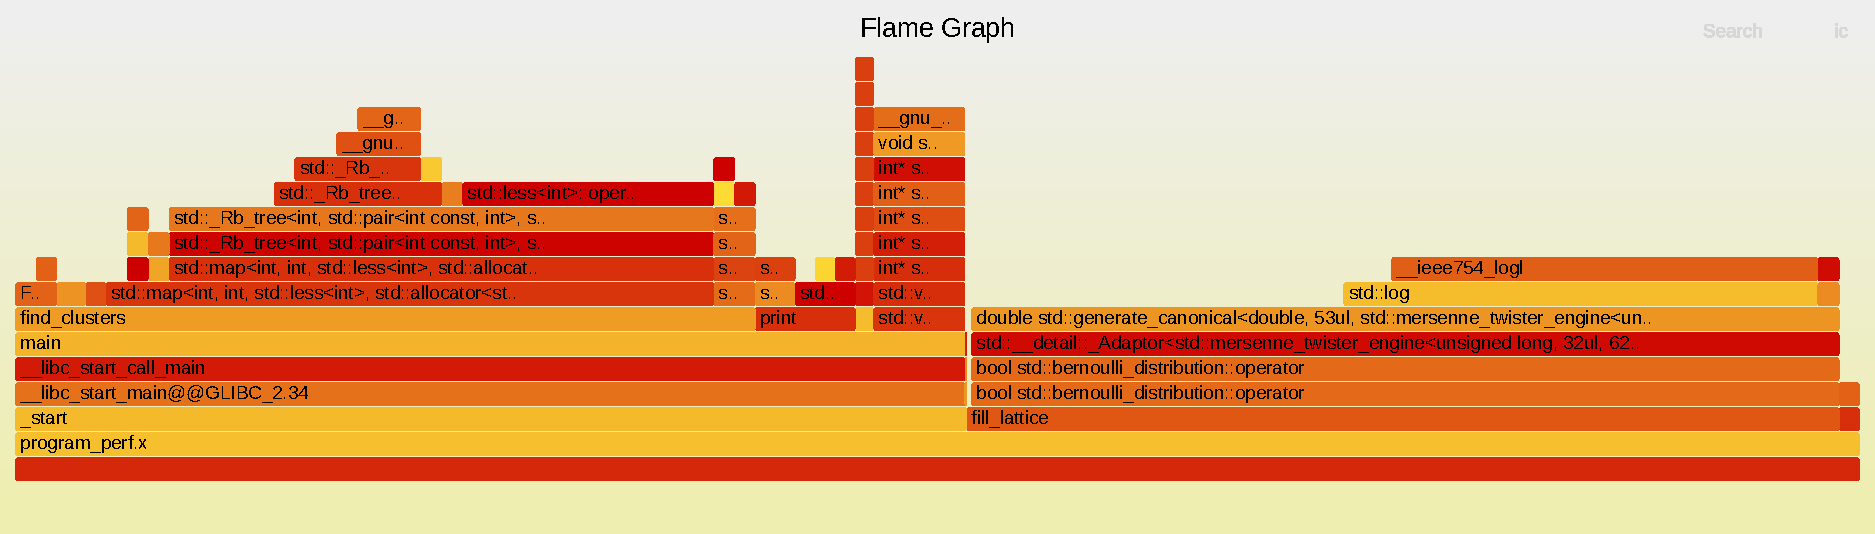
\includegraphics[width=1.0\textwidth]{figures/flamegraph.pdf}
    \caption{Flamegraph del perfil de ejecución generado con \texttt{perf}.}
    \label{fig:flamegraph}
\end{figure}

(COMPLETAR ANÁLISIS FLAMEGRAPH...)
  
Por otro lado se realizó un informe detallado de profiling obtenido con \texttt{gprof}, sin embargo, debido al uso de librerías sobre las cuales no tenemos control, era díficil obtener información. De esta manera se filtó el reporte para mostrar únicamente las funciones definidas en el código del proyecto, este incluye en el Anexo~\ref{app:flat_profile}. Cómo se puede observar tras el filtro, las funciones creadas corresponden a menos del 10\% del tiempo de ejecución. Por lo tanto, concluimos que el algoritmo utilizado es sumamente eficiente y la mayoría del tiempo se consume en las llamadas a funciones de la librería estandar de c++. 

\section{Optimizaciones realizadas}

El análisis del reporte de profiling mostró que las funciones definidas en nuestro código consumen un porcentaje muy bajo del tiempo total, por lo que no se identificaron optimizaciones significativas a través de gprof. Sin embargo, al examinar las gráficas de tiempos de ejecución con distintos niveles de compilación y revisar detenidamente el código, detectamos algunas mejoras puntuales: en lugar de inicializar el vector de etiquetas con un tamaño fijo de \(L^2/2\) y llenarlo, resultó más eficiente usar \texttt{$labels.push_back()$} dado que el número real de etiquetas es generalmente mucho menor que \(L^2/2\). Asimismo, la obtención de \texttt{$unique_ids$} se cambió de operar sobre la matriz completa a utilizar directamente el vector \texttt{labels}, más pequeño y suficiente para nuestro propósito. Finalmente, en la función de \texttt{Find} se implementó la rutina de compresión de camino, permitiendo que en llamadas porteriores se encontrara el cluster padre un poco más rapido, esto es especialmente util dado que es la función que más veces se llama en el codigo cómo lo demuestra el reporte de\texttt{gprof} . El código mencionado se observa en el Listing \ref{lst:opt_codigo_sin_acentos}. 
 
\begin{lstlisting}[language=C++,caption={Codigo de optimizaciones}, label={lst:opt_codigo_sin_acentos}]
    // ------------ Funcion HoshenKopelman: ------------
    //   Inserta nueva etiqueta en el vector de labels
    labels.push_back(next_label);
    
    // ------------ Funcion find_clusters: ------------
    //   Crea un unique_ids con vec labels en lugar de lattice 
    std::set<int> unique_ids(labels.begin(), labels.end()); 

    // ------------ Funcion Find: ------------
    //   Compresion de camino en union-find
    while (parent[ii] != ii) {
        kk = parent[ii];
        parent[ii] = jj;
        ii = kk;
    }
\end{lstlisting}


\section{Conclusiones}
...

\clearpage
\appendix
\section{Anexos}

\subsection{Flat profile de \texttt{gprof} filtrado}
\label{app:flat_profile}

A continuación se presenta el perfil plano (flat profile) generado por \texttt{gprof}, filtrado para mostrar únicamente las funciones definidas en el código del proyecto (se han eliminado entradas de librerías del sistema).

\lstinputlisting[caption={Flat profile filtrado de gprof},label={lst:gprof_filtered}]{out_report/report_gprof_filtered.txt}

\end{document}
